\documentclass[a4paper,french,10pt]{article}
\usepackage[utf8]{inputenc}
\usepackage[french]{babel}
\usepackage{graphicx}
\usepackage{float}
\addtolength{\oddsidemargin}{-2,5cm}
\addtolength{\textwidth}{5cm}
\addtolength{\topmargin}{-2,5cm}
\addtolength{\textheight}{4cm}

\title{\textbf{TALN -- Extraction à base de règles\\ \normalsize Extraction automatique de dates de soumission dans un corpus d'appels à contribution}}
\author{Thibaut \textsc{Marmin} \and Clément \textsc{Sipieter}}
\date{31 Mai 2011}

\begin{document}

\maketitle

\emph{Nous avons fait le choix de développer une commande permettant, à partir d'un message texte (par exemple un email et son header), de retourner la liste des dates contenues dans ce dernier. Chacune est couplée à une note de confiance, située entre zéro et un.}

\section{Utilitaire de séparation}
Un premier utilitaire de pré-traitement à été développé. Il permet simplement, à partir du fichier de corpus complet, de stocker chaque email dans un fichier texte différent.

Les fichiers générés contiennent l'entête de l'email et le message. L'entête sera filtrée par la suite lors de la recherche de dates.

\section{Utilitaire de recherche de dates}
Dans le but de pouvoir réutiliser notre application, nous avons fait le choix de développer une simple commande, prenant en entrée un email avec son entête sous la forme d'une chaine de caractères, et retourne la liste des dates de soumission associées à une note de confiance.

\begin{figure}[H]
\centering
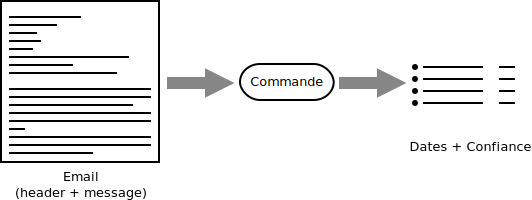
\includegraphics[width=0.6\textwidth]{files/archi}
\caption{Entrée / Sortie de la commande}
\end{figure}

\end{document}
